% No preâmbulo: \usepackage{graphicx,subfigure,placeins}
% Os painéis TLS atualizados ficam em figuras/continuidade/artigo/.
\FloatBarrier
\section{Avaliação e Resultados}
\label{sec:result}

A avaliação compreende experimentos de falhas de estado, interrupções do protocolo e recuperação com TLS nativo no Mininet-WiFi. O protótipo utiliza ML-KEM-512, ML-DSA-44 e AES-256-GCM. Os estudos de caso TLS comparam as configurações clássica, híbrida e pós-quântica descritas na Seção~\ref{sec:proposta}. As comparações de bytes são internas a cada implementação, cujos protocolos e parâmetros diferem. As configurações e os procedimentos de reprodução estão descritos na documentação dos experimentos.

\subsection{Falhas de Estado e Não Reutilização da Combinação de Chave e Nonce}

O primeiro experimento reúne 240 execuções: seis políticas, quatro falhas e dez repetições, com oito leituras antes e oito após reinício. Comparam-se restauração de checkpoint, persistência de contador por uso, reserva de blocos e três modos com chaves novas: completo pós-quântico, PSK e PSK+KEM. As falhas são reinício com checkpoint atual, queda de energia modelada, restauração de estado antigo e checkpoint truncado. As 65 verificações funcionais passaram, incluindo a detecção das falhas esperadas nos controles vulneráveis.

\begin{figure}[!htbp]
\centering
\setcounter{subfigure}{0}
\subfigure[Queda de energia modelada.]{
\label{fig:estado_energia}
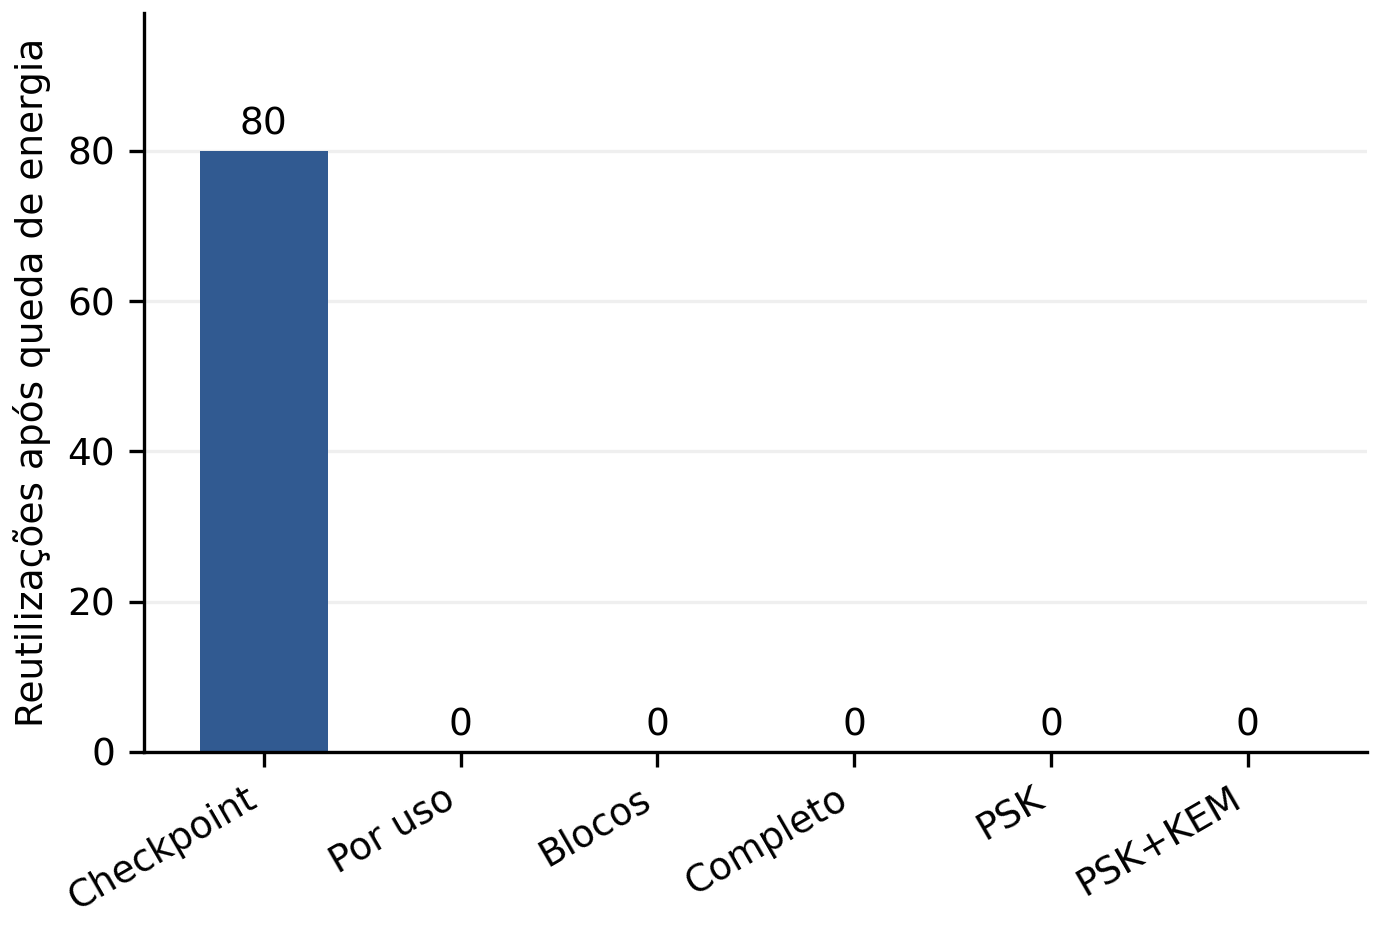
\includegraphics[width=0.46\linewidth]{figuras/avaliacao/estado_energia.png}
}
\hfill
\subfigure[Rollback do armazenamento.]{
\label{fig:estado_rollback}
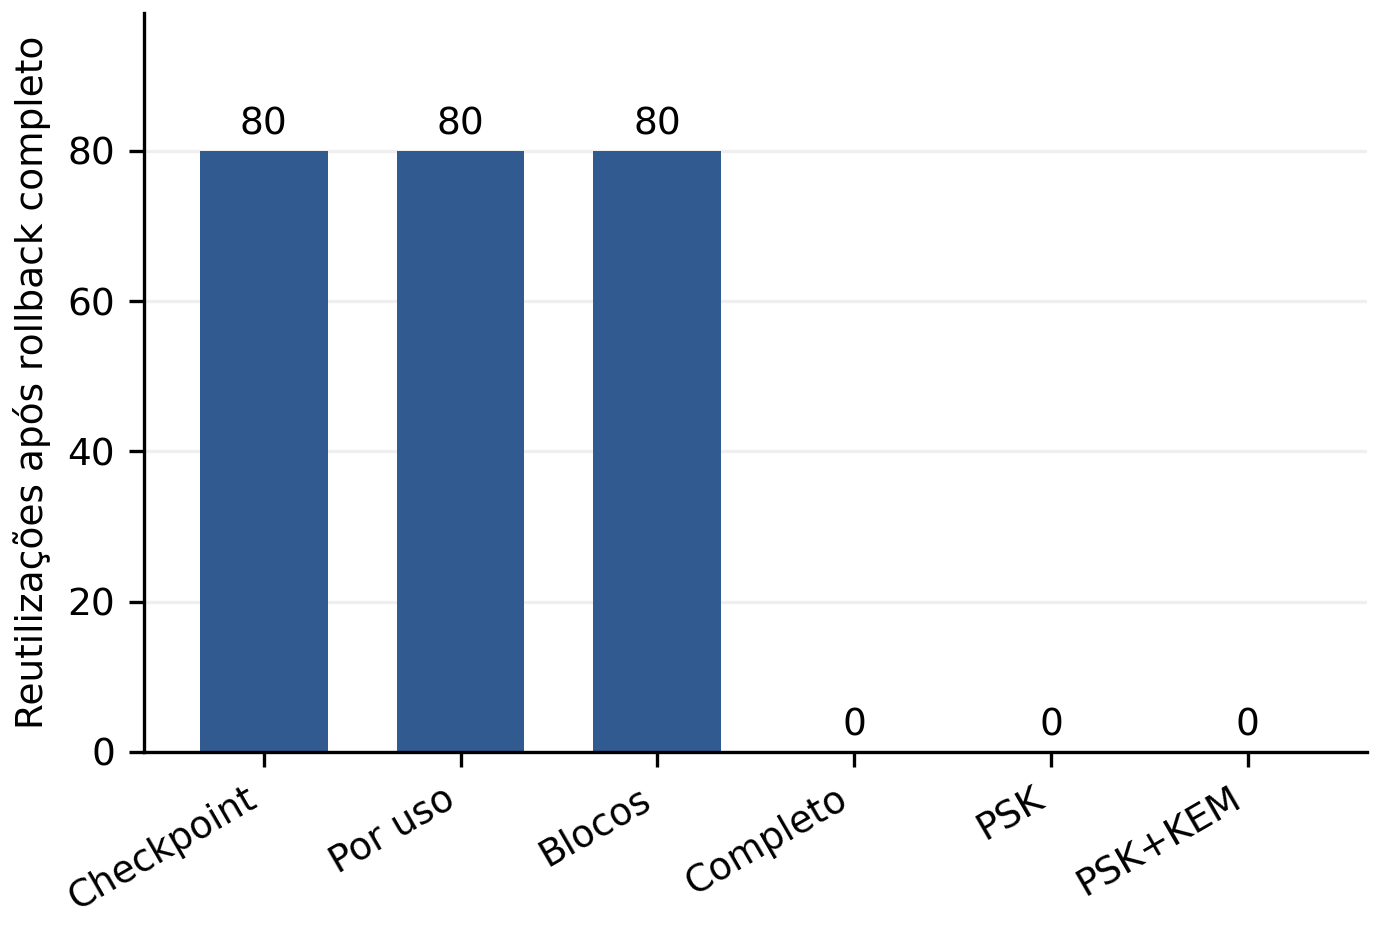
\includegraphics[width=0.46\linewidth]{figuras/avaliacao/estado_rollback.png}
}
\par\smallskip
\subfigure[Textos recuperados no rollback.]{
\label{fig:estado_textos}
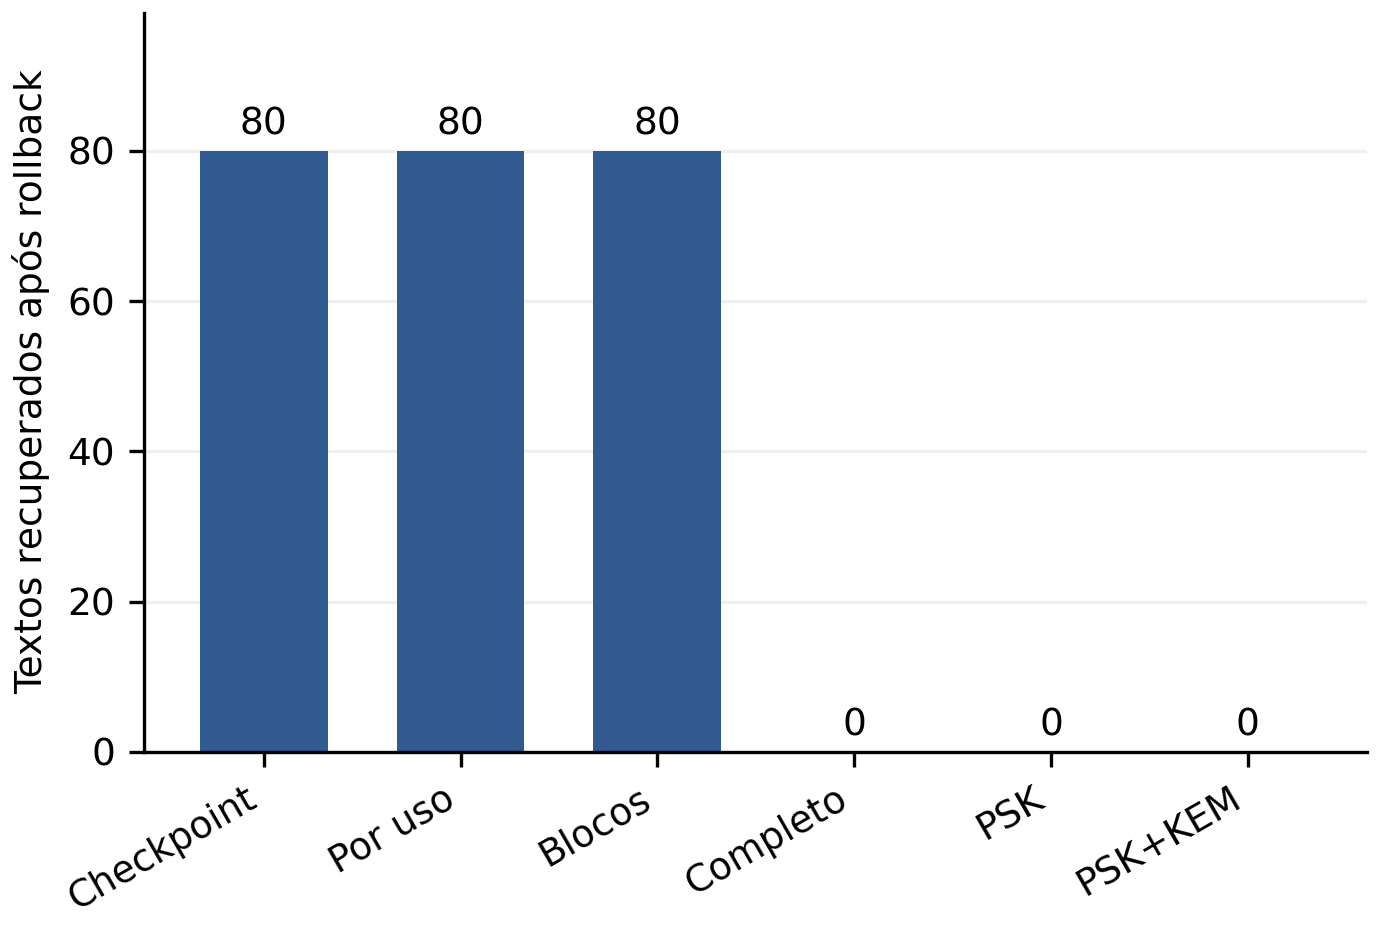
\includegraphics[width=0.46\linewidth]{figuras/avaliacao/estado_textos.png}
}
\hfill
\subfigure[Escritas na fase estável.]{
\label{fig:estado_escritas}
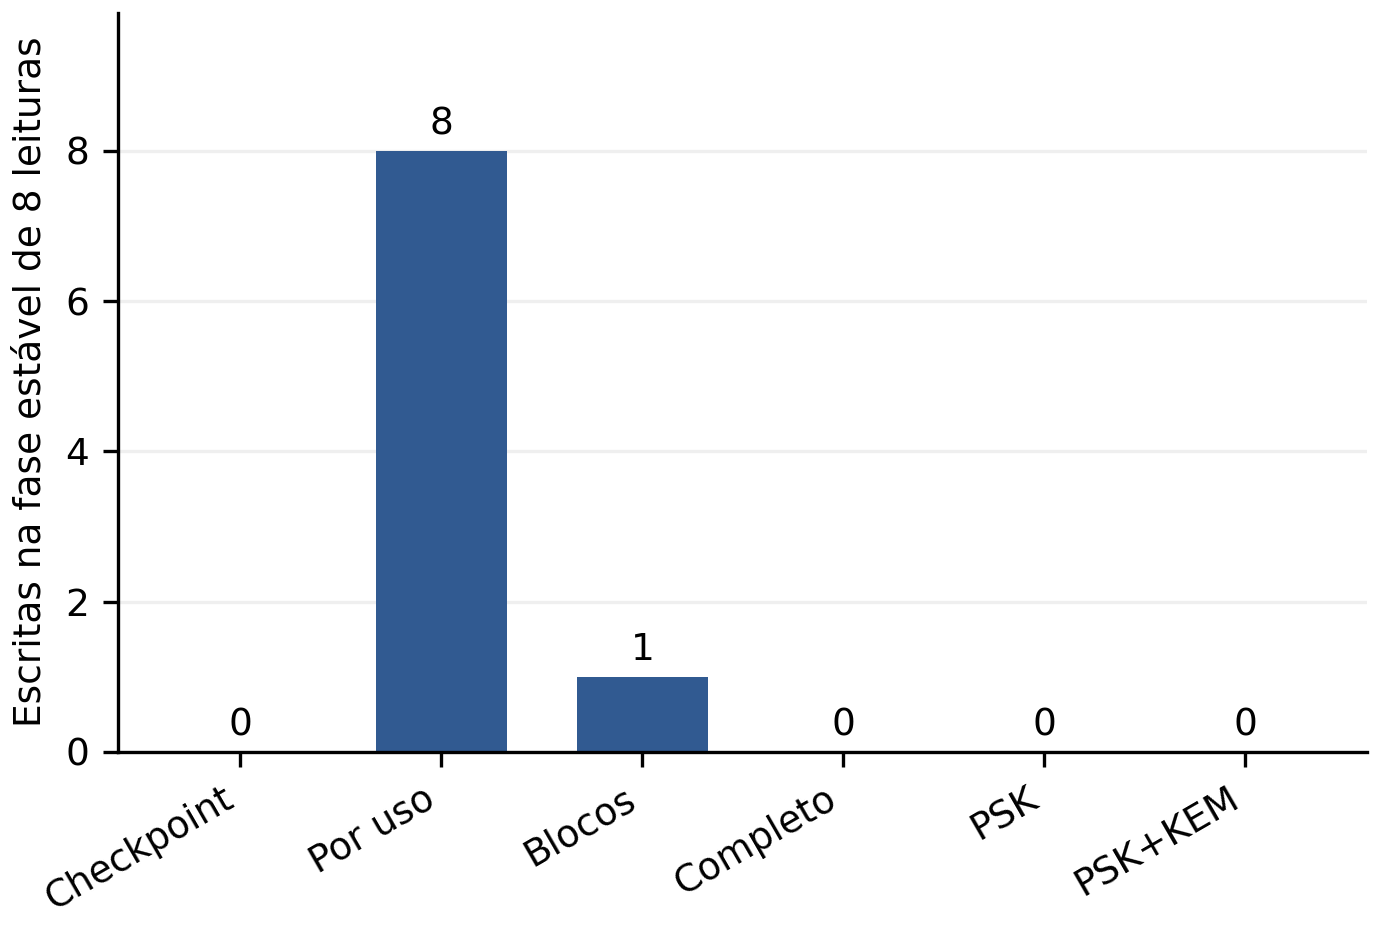
\includegraphics[width=0.46\linewidth]{figuras/avaliacao/estado_escritas.png}
}
\caption{Falhas de estado: (a--c) totais de dez execuções com oito leituras após a falha; (d) mediana de escritas nas oito leituras estáveis. A reserva utiliza blocos de 32 posições.}
\label{fig:estado_resultados}
\end{figure}

Na Figura~\ref{fig:estado_resultados}(a), o checkpoint antigo produziu 80 reutilizações da combinação de chave e nonce após a queda de energia modelada. Persistência por uso e reserva de blocos evitaram essa ocorrência com o registro atualizado dos contadores. Ao restaurar também esse registro, as três políticas de contador apresentaram 80 reutilizações cada, conforme a Figura~\ref{fig:estado_resultados}(b). Os modos com chaves novas não apresentaram reutilizações nos cenários testados.

O controle de texto conhecido recuperou 80 leituras por política vulnerável após a restauração do armazenamento (Figura~\ref{fig:estado_resultados}(c)). A rejeição pelo gateway não impediu a exposição no tráfego cifrado. Nas oito leituras estáveis, a persistência por uso realizou oito escritas, contra uma na reserva em blocos, excluindo inicialização e checkpoints do início da execução (Figura~\ref{fig:estado_resultados}(d)). A proteção dos contadores depende, portanto, de conservar seu registro atualizado.

\subsection{Interrupções, Fallback e Confirmação Perdida}

O segundo experimento reúne 330 casos: onze cenários, três modos com chaves novas e dez repetições. Os pontos A--K da Figura~\ref{fig:transicoes_resultados} representam: A, execução sem falha; B--H, interrupções após ClientHello, ServerHello, ClientFinished, atualização do estado do gateway, confirmação da chave, salvamento do checkpoint e cifragem da leitura, respectivamente; I, confirmação da leitura perdida; J, checkpoint truncado; e K, perda do segredo de retomada no gateway. O transporte é lógico, com primitivas criptográficas reais, e não representa perda de pacotes.

\begin{figure}[!htbp]
\centering
\setcounter{subfigure}{0}
\subfigure[Bytes por ponto de interrupção.]{
\label{fig:transicoes_bytes}
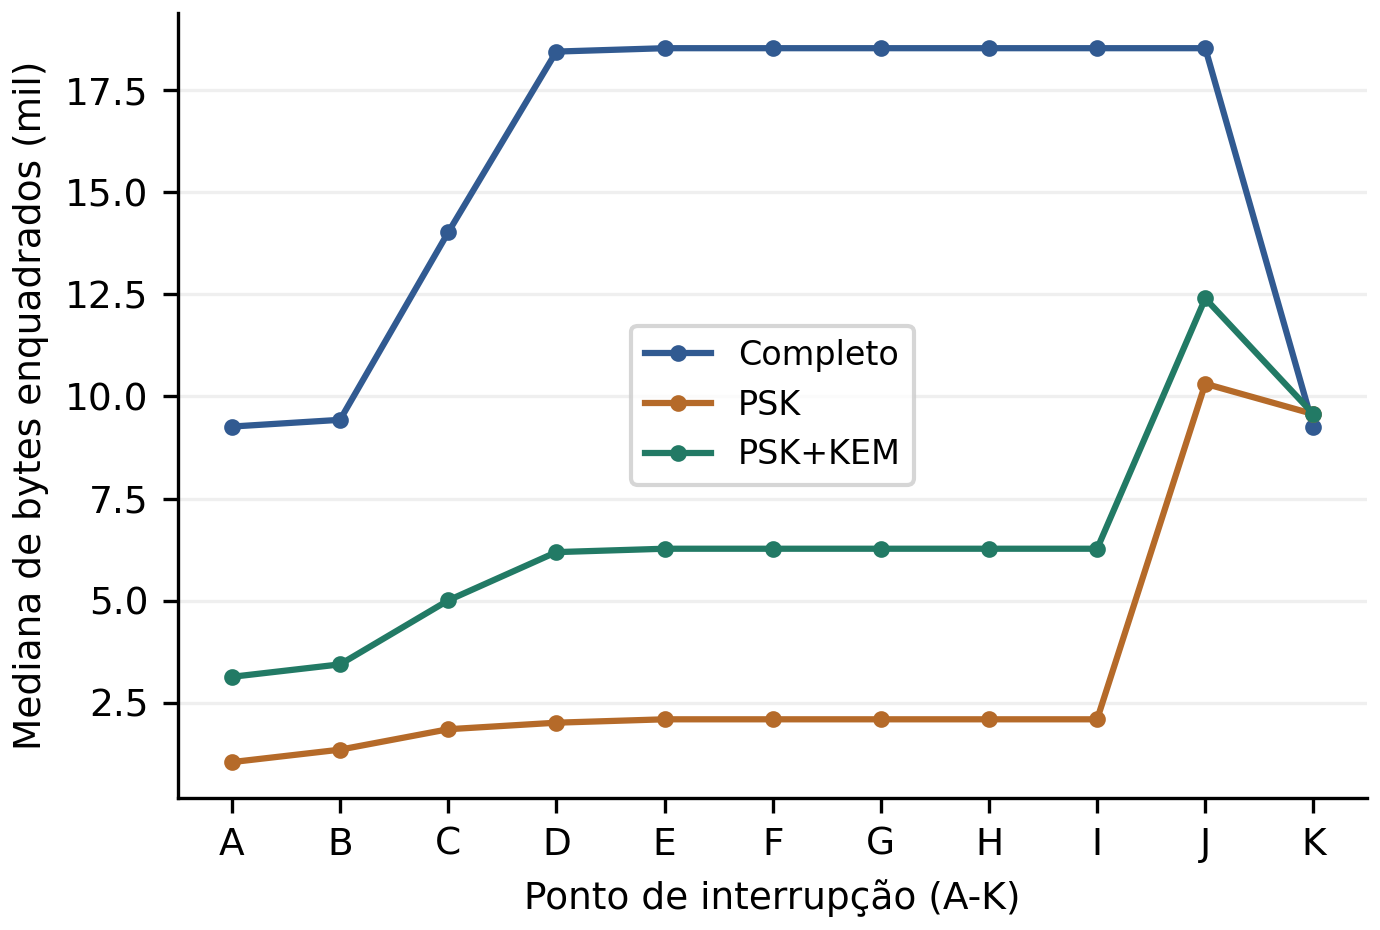
\includegraphics[width=0.46\linewidth]{figuras/avaliacao/transicoes_bytes.png}
}
\hfill
\subfigure[Autenticações completas com PSK+KEM.]{
\label{fig:transicoes_fallbacks}
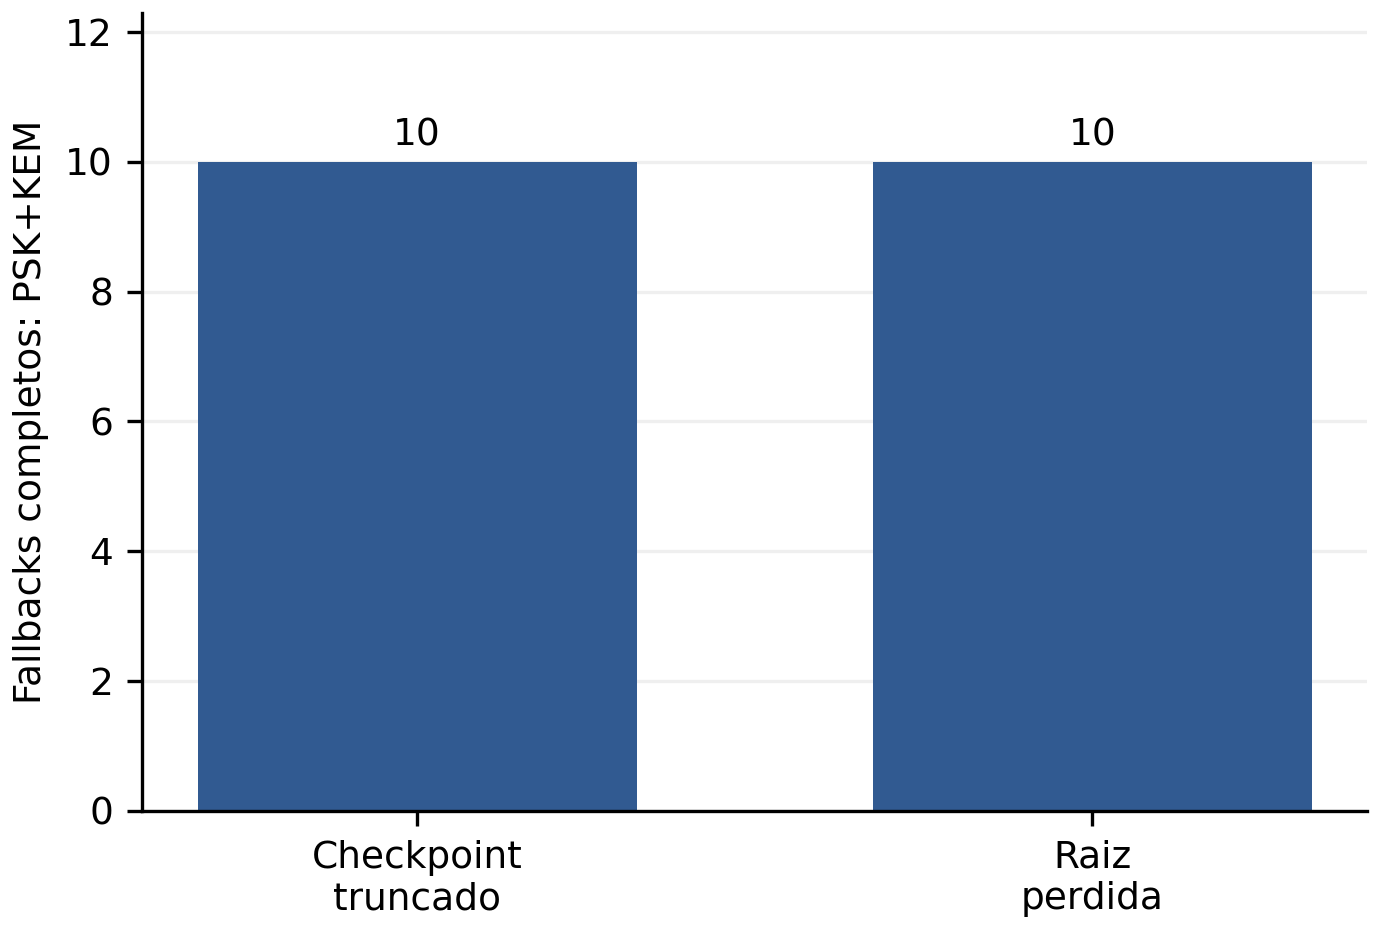
\includegraphics[width=0.46\linewidth]{figuras/avaliacao/transicoes_fallbacks.png}
}
\par\smallskip
\subfigure[Economia condicionada ao estado.]{
\label{fig:transicoes_economia}
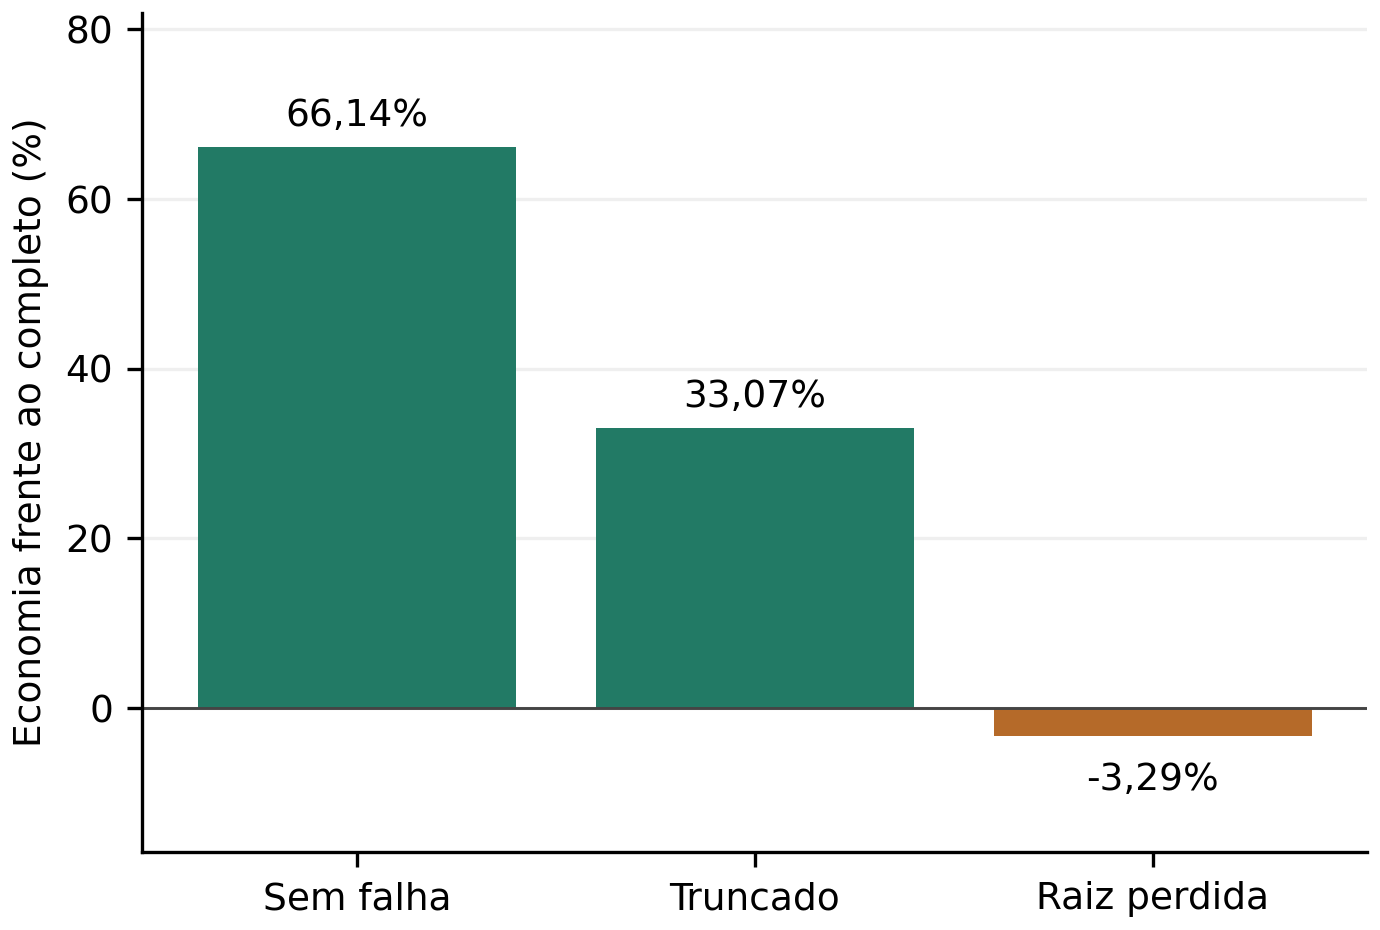
\includegraphics[width=0.46\linewidth]{figuras/avaliacao/transicoes_economia.png}
}
\hfill
\subfigure[Duplicação após confirmação perdida.]{
\label{fig:transicoes_duplicados}
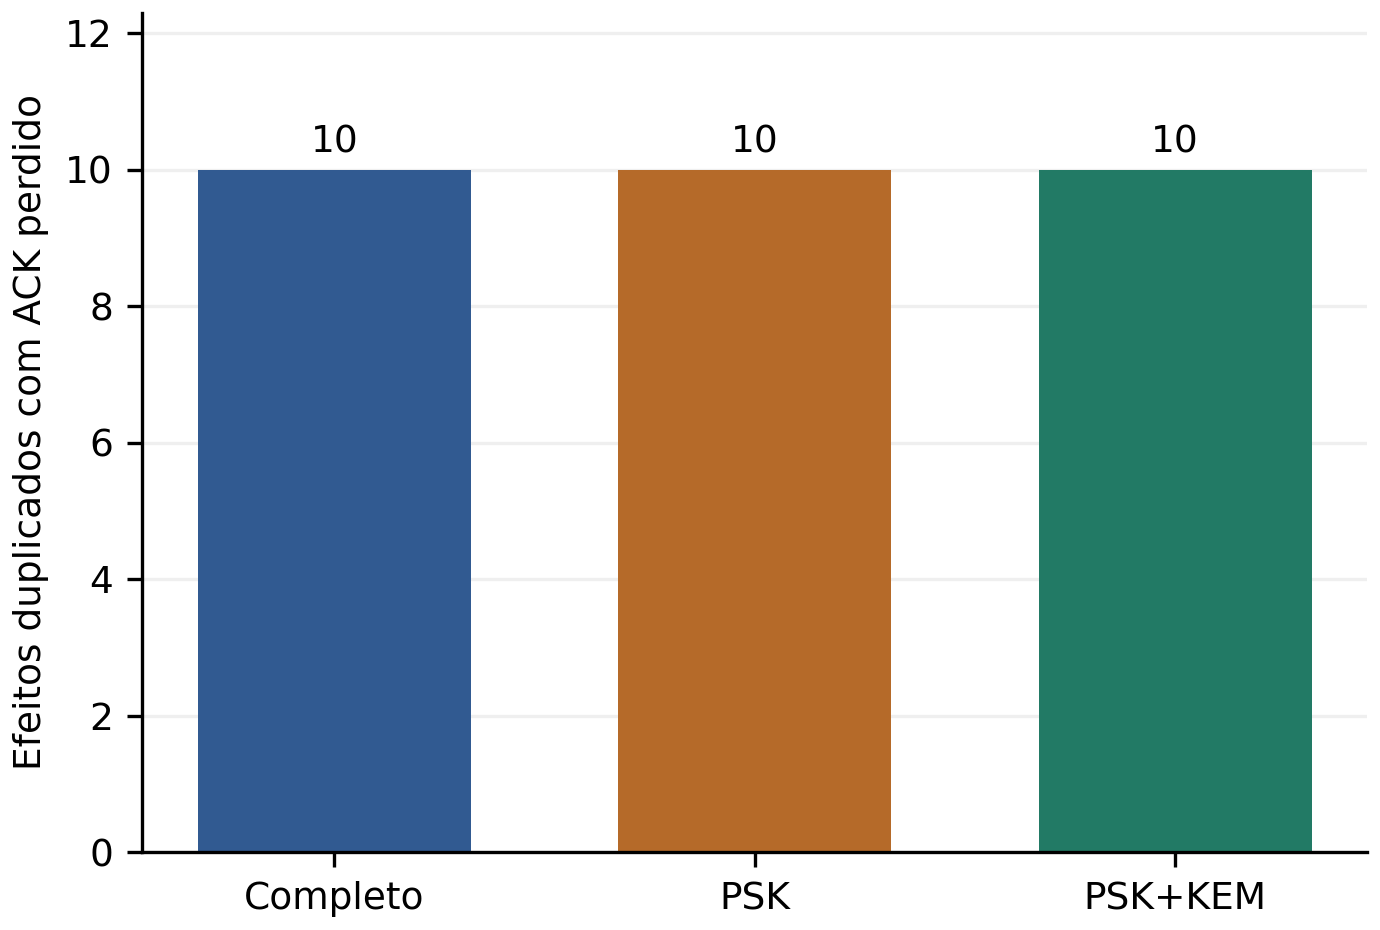
\includegraphics[width=0.46\linewidth]{figuras/avaliacao/transicoes_duplicados.png}
}
\caption{Interrupções no protótipo: medianas de dez repetições para bytes e economia; totais para autenticações completas e efeitos duplicados. A--K são definidos no texto. Esses bytes não representam TLS.}
\label{fig:transicoes_resultados}
\end{figure}

Sem falha, completo e PSK+KEM custaram 9.263 e 3.136 bytes, redução de 66,14\%. Com checkpoint truncado, os custos foram 18.526 e 12.399 bytes, redução de 33,07\%. Com o segredo de retomada perdido, a tentativa recusada seguida de autenticação completa custou 9.568 bytes, contra 9.263 do modo completo: acréscimo de 3,29\%. A economia depende, assim, do caminho de recuperação (Figura~\ref{fig:transicoes_resultados}(a--c)).

A contabilização inclui mensagens enquadradas das tentativas e confirmações perdidas; exclui preparação inicial, leituras e cabeçalhos IP. O transporte não envia uma mensagem de erro para o pedido rejeitado. Os modos com chaves novas atenderam aos critérios de não reutilização da combinação de chave e nonce e de recuperação após uma falha seguida de tentativa sem interrupção. Entretanto, a confirmação perdida produziu dez efeitos duplicados por modo sem supressão de repetições (Figura~\ref{fig:transicoes_resultados}(d)). O reconhecimento do efeito anterior depende do histórico da aplicação.

\subsection{Recuperação com TLS Clássico e Pós-Quântico}
\label{sec:continuidade_tls}

Os estudos de caso comparam autenticação completa direta, retomada com chave dos tickets perdida no reinício e retomada com essa chave preservada. Cada tratamento é executado nas três configurações criptográficas, mantendo TLS 1.3, autenticação mútua, AES-256-GCM/SHA-384, aplicação e carga. As duas políticas de retomada utilizam a mesma construção de tickets sem cache por sessão. As cadeias transmitidas pelo servidor incluem o certificado folha e a CA raiz nos três perfis.

Cada execução contém nove leituras: uma inicial sem falha e oito elegíveis. Reinícios do gateway e supressões da primeira confirmação ocorrem em 0\%, 25\% ou 100\% das leituras elegíveis, podendo coincidir. Assim, 25\% corresponde a duas dessas oito leituras. A conexão é interrompida após a gravação e antes da confirmação, e o reenvio conserva o identificador. Há até três tentativas por leitura, com limite de 95 s por processo; entregas não concluídas são mantidas nos dados. As agendas são iguais entre os comparadores de cada bloco, cuja ordem é aleatorizada.

A matriz principal reúne 1.620 execuções: três frequências de reinício, três de confirmação perdida, três perfis, três tratamentos, dois modos de deduplicação e dez blocos, sob perda de pacotes configurada em 0\%. Outros 180 casos usam perdas de 1\% e 5\%, com reinícios e confirmações perdidas em 25\% e deduplicação ativa. As perdas do kernel não são exatamente pareadas entre comparadores.

O ambiente utiliza Intel Core i5-8365U, quatro núcleos e oito threads, aproximadamente 16 GB de RAM, contêiner Ubuntu 22.04.5, Python 3.10.12 e OpenSSL 3.5.9. O Mininet-WiFi conecta um sensor emulado, um ponto de acesso e o gateway. O enlace AP--servidor recebe atraso de 2 ms por direção, fila de 1.000 pacotes e as perdas configuradas, sem limite de taxa no netem.

Os bytes IPv4 abrangem todas as tentativas e encerramentos da sequência observados no servidor. O custo por leitura confirmada divide esse total pelo número de leituras confirmadas. O tempo termina na última confirmação e inclui processos, reinícios previstos e reenvios; divide-se pela quantidade de leituras da sequência. Preparação da rede, credenciais e distribuição inicial da chave dos tickets ficam fora da medição. A unidade de repetição é o bloco. As comparações são realizadas dentro da mesma repetição, utilizando o modo completo do mesmo perfil como referência. As economias apresentadas são as medianas das reduções percentuais calculadas nos blocos. Os intervalos bootstrap de 95\%, com 10.000 reamostragens, são exploratórios por configuração.

\begin{figure}[!htbp]
\centering
\setcounter{subfigure}{0}
\subfigure[Bytes por leitura com falhas em 100\%.]{
\label{fig:tls_custos}
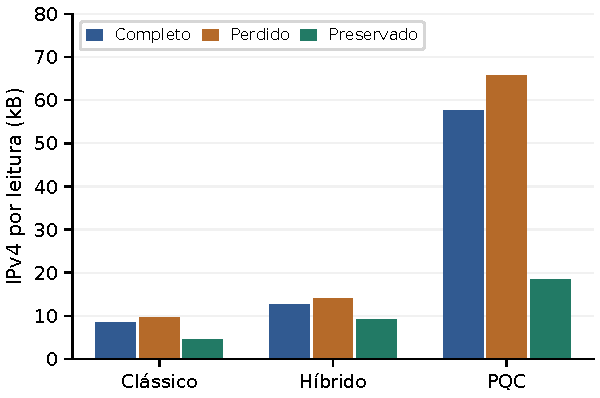
\includegraphics[width=0.47\linewidth]{figuras/continuidade/artigo/tls_custos.pdf}
}
\hfill
\subfigure[PQC: política e frequência de falhas.]{
\label{fig:tls_economia}
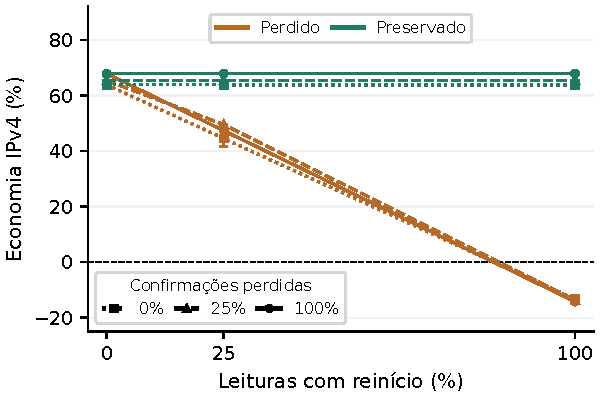
\includegraphics[width=0.47\linewidth]{figuras/continuidade/artigo/tls_economia.pdf}
}
\par\smallskip
\subfigure[PQC preservado: tempo sob perdas.]{
\label{fig:tls_tempo}
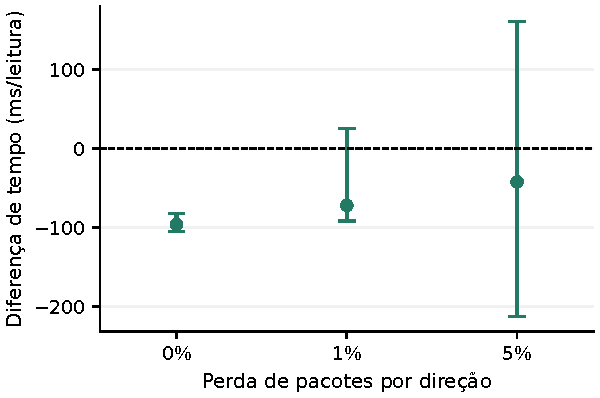
\includegraphics[width=0.47\linewidth]{figuras/continuidade/artigo/tls_tempo.pdf}
}
\hfill
\subfigure[PQC: handshakes com falhas em 100\%.]{
\label{fig:tls_handshakes}
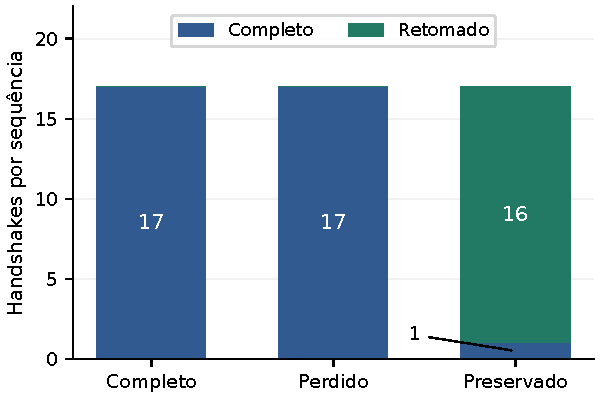
\includegraphics[width=0.47\linewidth]{figuras/continuidade/artigo/tls_handshakes.pdf}
}
\par\smallskip
\subfigure[Tamanho da identidade de retomada.]{
\label{fig:tls_identidade}
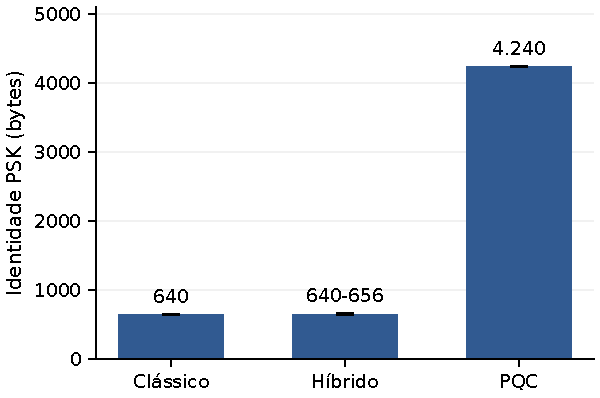
\includegraphics[width=0.47\linewidth]{figuras/continuidade/artigo/tls_identidade.pdf}
}
\hfill
\subfigure[Efeitos duplicados na matriz principal.]{
\label{fig:tls_duplicacoes}
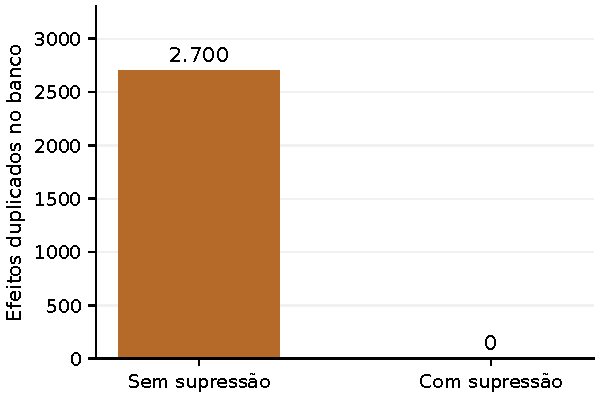
\includegraphics[width=0.47\linewidth]{figuras/continuidade/artigo/tls_duplicacoes.pdf}
}
\caption{Recuperação TLS: (a, d) medianas de dez blocos, com reinícios e confirmações perdidas em 100\% das leituras elegíveis; (b) economia calculada dentro de cada bloco no PQC; (c) diferença temporal frente ao completo, com falhas lógicas em 25\%; (e) medianas e faixas observadas; (f) totais de 810 execuções e 7.290 leituras por modo de deduplicação. Em (a--d), deduplicação ativa; em (a, b, d), perda de pacotes configurada em 0\%. Hastes em (b, c) são intervalos bootstrap exploratórios de 95\%.}
\label{fig:tls_resultados}
\end{figure}

A Figura~\ref{fig:tls_resultados}(a) apresenta os custos com reinícios e confirmações perdidas em todas as leituras elegíveis. No PQC, as medianas foram 57.489,44 bytes por leitura no completo, 65.673,67 com contexto perdido e 18.469,00 com preservação. As comparações realizadas dentro da mesma repetição indicaram aumento de 14,24\% [14,15; 14,31] no contexto perdido e economia de 67,87\% [67,86; 67,90] com preservação. No clássico, houve aumento de 14,91\% e economia de 45,07\%, respectivamente; no híbrido, aumento de 11,31\% e economia de 28,42\%. O problema também ocorre com criptografia clássica.

Na Figura~\ref{fig:tls_resultados}(b), a economia PQC com reinícios e confirmações perdidas em 25\% foi de 49,56\% com contexto perdido e 65,43\% com preservação. As linhas ligam somente as três frequências medidas, sem estabelecer um limiar para valores intermediários. Na comparação temporal com contexto preservado (Figura~\ref{fig:tls_resultados}(c)), as diferenças por leitura foram -96,06 ms [-105,57; -82,62], -72,09 ms [-91,75; 24,92] e -42,32 ms [-212,56; 160,62] sob perdas de 0\%, 1\% e 5\%. Os intervalos em 1\% e 5\% incluem zero. A economia de bytes permaneceu em 65,43\% e 65,45\% nesses dois cenários, sem demonstrar superioridade temporal geral.

A Figura~\ref{fig:tls_resultados}(d) explica o cenário de falhas frequentes no PQC: completo e contexto perdido executaram 17 handshakes completos, contra um completo e 16 retomados com preservação. Após a interrupção abrupta, a tentativa completa não deixou uma sessão substituta utilizável no cliente. Com a chave perdida, o ticket antigo continuou inválido no reenvio. Essa observação descreve a disponibilidade da sessão no cliente, sem afirmar ausência de tickets enviados pelo servidor.

A análise posterior dos 21.960 ClientHello mediu identidades PSK de 640 bytes no clássico, 640--656 no híbrido e 4.240 no PQC (Figura~\ref{fig:tls_resultados}(e)). No PQC, a extensão de retomada acrescentou 4.303 bytes ao ClientHello. Quando o ticket é recusado, esse material acompanha a conexão que realiza autenticação completa. Foram medidos apenas comprimentos públicos, sem decifrar tickets. As diferenças de codificação e implementação limitam a atribuição de cada byte a uma primitiva isolada.

Todas as 16.200 leituras foram confirmadas em 21.960 tentativas. Na matriz principal, houve zero efeitos duplicados com deduplicação e 2.700 sem supressão (Figura~\ref{fig:tls_resultados}(f)); cada modo contém 810 execuções e 7.290 leituras. Os 180 casos adicionais com deduplicação também apresentaram zero duplicações. Esse resultado depende do histórico atualizado e dos efeitos gravados na mesma operação do banco.

Os percentuais valem para as cadeias avaliadas, que incluem a CA raiz; omiti-la pode alterar o custo completo e a economia, especialmente com ML-DSA. Essa variante ainda não foi medida. Blocos interrompidos por indisponibilidade da infraestrutura ou descarte na captura foram refeitos integralmente; os incluídos atenderam ao critério de zero descartes, com procedência registrada. Dez blocos, um sensor e um host compartilhado delimitam a avaliação. Tempos e escritas no host não medem energia ou desgaste de sensores físicos, e os resultados não abrangem rollback conjunto nem execução única de atuadores externos.

\FloatBarrier
